%!TEX root = ./main.tex


\begin{frame}
  \centering
  \Huge
  \textbf{My View on AI}\\
  \vspace{1em}
  \large
      Can we use \textbf{ChatGPT, Claude, Gemini, Copilot, etc.} \\ to help with assignments?
\end{frame}

\begin{frame}
  \begin{columns}
    \column{0.45\textwidth}
      \Huge
      Absolutely!
    \column{0.55\textwidth}
      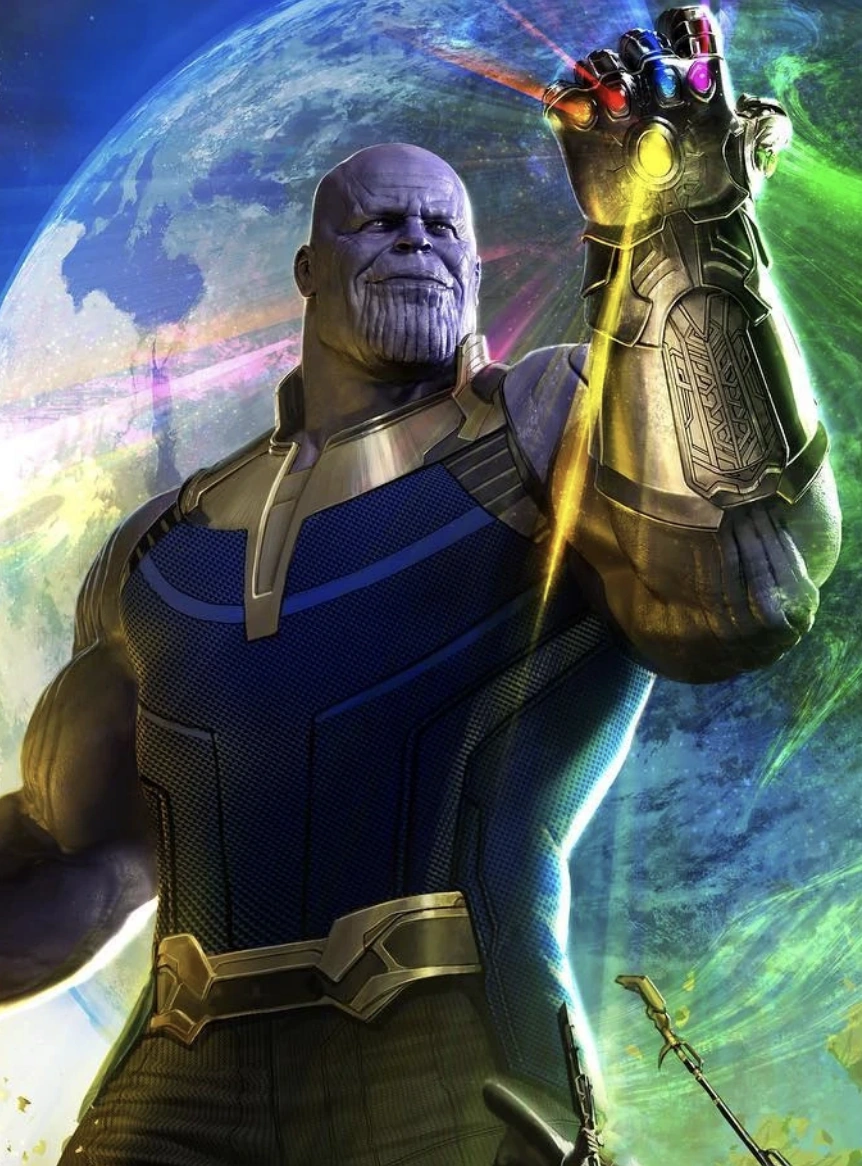
\includegraphics[width=\linewidth]{figure/thanos.png}
  \end{columns}
\end{frame}



\begin{frame}{Use It!}
    \large
    \begin{itemize}
        \item You're welcome to use AI tools to brainstorm, generate code, or write explanations.
        \item You can even include notes like “This answer was inspired by ChatGPT 5.6 Sol” — that's fine.
        \item I want you to learn how to use AI productively, just like in real-world engineering.
    \end{itemize}
\end{frame}

\begin{frame}{But Outsmart It.}  

\Large    
\begin{itemize}
    \item My job is to make sure assignments are designed so that AI won’t give you perfect answers easily.
    \item Your real skill is not in copying the AI's answer— it's in understanding, adapting, and improving what AI gives you.
\end{itemize}

\vspace{1em}

\LARGE
\centering
\textcolor{red}{\textbf{\textit{AI is welcome. Lazy copying is not.}}}

\end{frame}

% \begin{frame}{The World Has Changed (cont'd)}

% \textbf{No one can stop China now}
% \begin{itemize}
%   \item The talent pipeline has reached a breakthrough point
%   \item No industry can hold back Chinese talent anymore
% \end{itemize}

% \vspace{1em}

% \textbf{Humanity has created something entirely new}
% \begin{itemize}
%   \item After prosperity, we may have to face existential questions...
%   \item Productivity gaps between people will become extreme
%   \begin{itemize}
%     \item \textcolor{blue}{The marginal return of test-driven “merit” and learning is rapidly shrinking}
%     \item AI has started to erode the value of top-tier “human labor”
%   \end{itemize}
% \end{itemize}

% \end{frame}

% \begin{frame}{We’ve Come a Long, Hard Way}

% \textbf{Everyone begins a new chapter in college}

% \begin{quote}
% \textcolor{blue}{But the first thing that hits you is a slap in the face:}
% "I once doubted if I was even fit for computer science,
% because every childhood fantasy I had about hacking 
% was crushed in my very first semester."  
% —— \href{https://csdiy.wiki}{CS Self-Study Guide}
% \end{quote}

% \begin{quote}
% Passionate and bright students… they’ve heard of relativity, quantum mechanics…
% But after slogging through the early courses (like vector calculus and electrostatics), 
% many just give up.  
% —— \textit{The Feynman Lectures on Physics}
% \end{quote}

% \vspace{1em}

% \textbf{Where is the person who lights up the dream in us?}

% \begin{quote}
% \textit{Education is not the filling of a pail, but the lighting of a fire}  
% —— William Butler Yeats
% \end{quote}

% \end{frame}


% \begin{frame}{Dream vs Reality: When I Started Teaching OS (AD 2018)}

% \textbf{Frontend programmers reshaped the open-source ecosystem}
% \begin{itemize}
%   \item ES5: 2009, React.js: 2013, VSCode: 2015, ...
%   \item “Programming” is no longer a privilege for a few geeks
% \end{itemize}

% \vspace{1em}

% \textbf{A perfect textbook finally appeared}
% \begin{itemize}
%   \item \href{https://pages.cs.wisc.edu/~remzi/OSTEP/}{\textit{Operating Systems: Three Easy Pieces}}
% \end{itemize}

% \vspace{1em}

% \textbf{After returning from the US, I saw where the bar is}
% \begin{itemize}
%   \item At least there's hope that we can live \textcolor{blue}{as well as foreigners}!
% \end{itemize}

% \vspace{1em}

% \textcolor{blue}{\textbf{But the first thing that hits you is a slap in the face:}}  
% The department made me sit behind my advisor’s chair as a TA to observe quietly…  
% Of course, such things would never be allowed to happen to someone with top honors like me!
% \end{frame}

% \begin{frame}{Dream vs Reality: When I Started Teaching OS (AD 2018)}

% \textbf{\textcolor{blue}{Altair 8800: The Machine That Launched the PC Revolution}}

% \begin{itemize}
%   \item In 1975, Bill Gates and Paul Allen implemented a full system emulator of the Altair 8800 
%         on a PDP-10 at Harvard, and wrote the first BASIC interpreter for it
%   \item With dreams (and punched tapes) in hand, they flew to MITS to demo it — and became legends
% \end{itemize}

% \vspace{1em}

% \textbf{It took us 40 years, but we made it!}
% \begin{itemize}
%   \item Today, anyone can build a full system emulator
%   \item We now have a great set of programming labs
% \end{itemize}

% \end{frame}



